\documentclass[12pt,a4paper]{article}

\setlength{\parindent}{0.1 in}
%\setlength{\parskip}{0.1 in}
\setlength{\oddsidemargin}{0.25 in}
\setlength{\evensidemargin}{-0.25 in}
\setlength{\topmargin}{-0.5 in}
\setlength{\textwidth}{7.0 in}
\setlength{\textheight}{9.5 in}
\setlength{\headsep}{0.45 in}

%\usepackage[fleqn]{amsmath}
%\usepackage{amsfonts,graphicx}
\usepackage{amsmath,amsfonts,graphicx}
\usepackage[fleqn]{mathtools}
\usepackage{setspace}
\usepackage{hyperref}
\usepackage[nottoc]{tocbibind}
\usepackage{tocloft}
\usepackage[outermargin=2 in]{geometry}
\usepackage{scrextend}
\usepackage{tensor}
\usepackage{cancel}
\usepackage{slashed}


%Adding `Appendix' to the appendices
\usepackage[toc,page]{appendix}

%Add a bullet point to description items
\usepackage{enumitem}

%Mathematics
\usepackage{braket}
\usepackage{ulem}
\usepackage{xcolor}
\usepackage[font={small,it}]{caption}

\bibliographystyle{unsrt}

%New commands
%Maths
\newcommand{\beq}{\begin{equation}}
\newcommand{\eeq}{\end{equation}}
\newcommand{\bea}{\begin{align}}
\newcommand{\eea}{\end{align}}
\newcommand{\p}{\partial}
\newcommand{\trace}[1]{\mathrm{Tr}\left[#1 \right]}
\newcommand{\ptrace}[2]{\mathrm{Tr}_{#1} \left[ #2 \right]}
\newcommand{\bpmat}{\begin{pmatrix}}
\newcommand{\epmat}{\end{pmatrix}}
\newcommand{\vv}[1]{\vec{#1}}
\newcommand{\mat}[1]{\uuline{#1}}
\newcommand{\norm}[1]{\| #1 \|}
\newcommand{\op}[1]{\mathbb{#1}}
\newcommand{\vhat}[1]{\hat{\vv{#1}}}

%Renewed commands, in order for them to take arguments with automatically adjusted brackets 
\renewcommand{\dim}[1]{\mathrm{dim}\left( #1\right)}
\renewcommand{\det}[1]{\mathrm{det} \left( #1 \right)}
\renewcommand{\exp}[1] {\mathrm{exp} \left[ #1 \right]}


%\mathbb Letters
\newcommand{\identity}{\mathbb{I}}
\newcommand{\inreal}{\mathbb{R}}
\newcommand{\incomplex}{\mathbb{C}}

%Redefine Braket
\renewcommand{\braket}[1]{\left\langle #1 \right\rangle}

%Integration
\newcommand{\intd} {\mathrm{d}}

%Operators
\newcommand{\phihat}{\hat{\phi}}
\newcommand{\xhat}{\hat{x}}
\newcommand{\phat}{\hat{p}}
\newcommand{\Dhat}{\hat{D}}
\newcommand{\Hhat}{\hat{H}}
\newcommand{\ahat}{\hat{a}}
\newcommand{\bhat}{\hat{b}}
\newcommand{\chat}{\hat{c}}
\newcommand{\Phihat}{\hat{\Phi}}

%Channels
\newcommand{\channel}[3]{\mathcal{#1}^{#2 \rightarrow #3}}


%Caligraphy letters
\newcommand{\cl}[1]{\mathcal{#1}}
\newcommand{\Hilbert}{\mathcal{H}}
\newcommand{\calN}{\mathcal{N}}
\newcommand{\Lag}{\mathcal{L}}
\newcommand{\calD}{\mathcal{D}}


%Pauli
\newcommand{\Xhat}{\hat{X}}
\newcommand{\Yhat}{\hat{Y}}
\newcommand{\Zhat}{\hat{Z}}
\newcommand{\PauliX}{\bpmat 0 & 1 \\ 1 & 0 \epmat}
\newcommand{\PauliZ} {\bpmat 1 & 0 \\ 0 & -1\epmat}



%Gell-Mann matrices
\newcommand{\GMone} {\bpmat 0 & 1 & 0 \\ 1 & 0 & 0 \\ 0 & 0 & 0 \epmat }
\newcommand{\GMsix}{\bpmat 0 & 0 & 0 \\ 0 & 0 & 1\\ 0 & 1 & 0\epmat}

%Density matrices
\newcommand{\rhotwo}{\bpmat 1 & e^{-it} \\ e^{it} & 1 \epmat}
\newcommand{\rhothree} {\bpmat 1 & e^{it} & e^{2it} \\
e^{-it} & 1 & e^{it} \\
e^{-2it} & e^{-it} & 1 \epmat}



%Misc
\def\dbar{{\mathchar'26\mkern-12mu d}} %a $d$ with a bar through its stem


\newcommand{\eq}[1]{$#1$}

%Undertilded quantities
\newcommand{\tildeq}{\underset{^\sim}q}
\newcommand{\tildep}{\underset{^\sim}p}

%Curly letters
\newcommand{\calE}{\mathcal{E}}

\newcommand{\Nhat}{\hat{N}}

%Wave vector shortening
\newcommand{\kvec}{\vv{k}}












\begin{document}
\title{Quantum Error Correction - Lecture 6}
\author{with Dan Browne}
\maketitle
\tableofcontents




Recall that we spoke about fault tolerant constructions. We want each component failure which occurs with probability $p$ to cause up to $c$ single errors in each code block. 

We must now consider:
\begin{itemize}
\item Unitary gates
\item State preparation
\item Measurements
\end{itemize}
The problem is that many constructions are based on CNOT gates. In this general error model, a CNOTfailing can cause a 2-qubit error. 

A CNOT inside a code block fails to meet the conditions of fault-tolerance. We can absolutely not have any instance of a CNOT gate inside a code block. 

So, we allow entangling gates on between code blocks. We call these \textbf{transversal gates}. A unitary gate is transversal if it contains no entangling gates within a code block. Let us look at the Steane code as an example. 

For a code block with seven qubits, and logical operators $\bar{X} = X^{\otimes7}$ and $\bar{Z} = Z^{\otimes 7}$. These do not entangle. If $\bar{X}$ and $\bar{Z}$ are transversal, then  $\bar{Y}$ is too since $\bar{Y} = i \bar{X} \bar{Z}$. The Steane code also has $\bar{H} = H^{\otimes 7}$. and $\bar{S} = (S¨\dagger)^{\otimes 7}$. 

Question: Why must we take the adjoint of the $S$ gate? 

However, for the Steane code, it turns out that we can create  a CNOT gate that is also transversal! 

\begin{figure}[h]
\centering
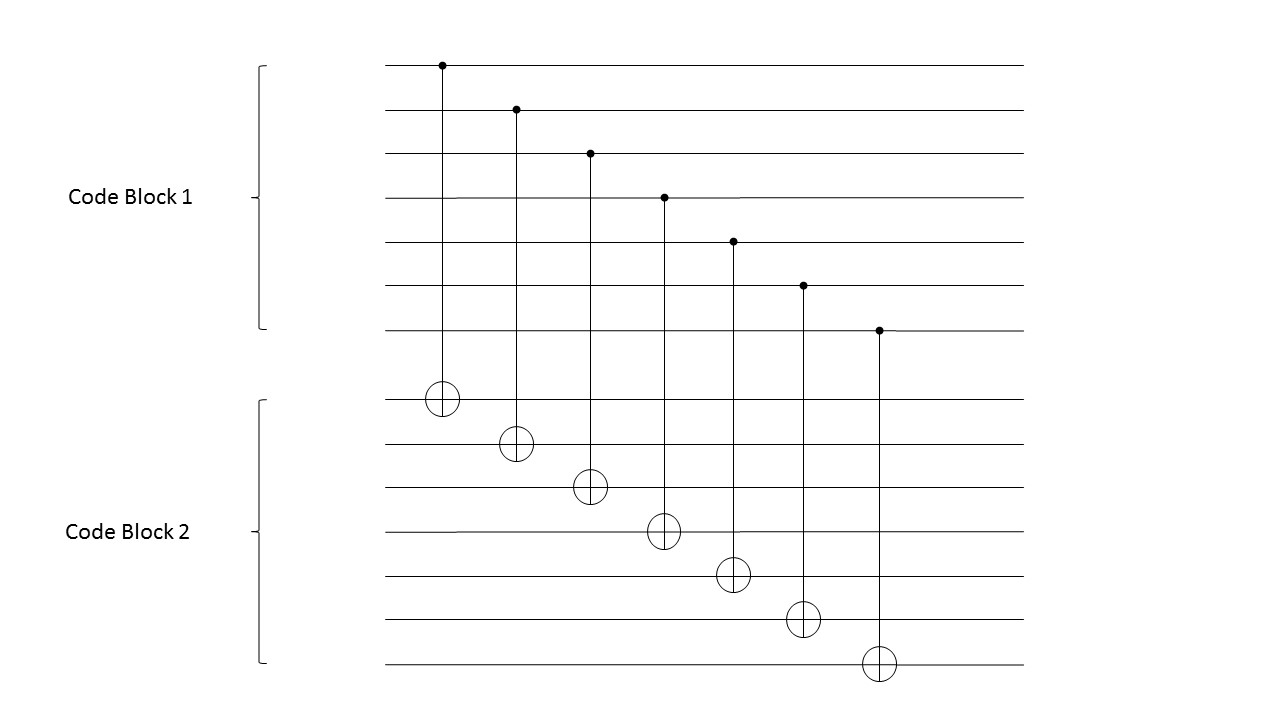
\includegraphics[width = \textwidth ]{./Transversal_CNOT.jpg}
\caption{Transversal CNOT gate.}
\end{figure}

We just have to make sure that every CNOT component acts between code blocks. But later, we will need universal gates. It turns out that the stabiliser formalism and transversal gates is not fault tolerant on its own. But recall that the Clifford group is fault tolerance. 

\section{Fault tolerant stabiliser measurement}
Recall our general Pauli tensor product projector that can be used as a measurement:
\beq
P = p_1 \otimes P_2 \otimes P_3 \ldots P_n
\eeq
Recall the phase kick-back circuit that we wanted. Each projector projects onto a qubit and the outcome is recoded in an ancilla. The ancilla doesn't need to be in the code block. However, an error on the ancilla means that it can propagate down. 

$Z$-errors would not propagate down, but $X$ errors would after the 1st gate. However, we can fix this with the repetition code. We can create a so-called cat-state. The trick is that for an ancilla, instead of $\ket{+}$, we use $\ket{0}^{\otimes n} + \ket{1} ^{\otimes n}$. This is GHZ state, but as mentioned is also called a cat-state. It is a repetition code implementation. 

\subsection{Example: 3-qubit code}
Given the ancilla state $\ket{000} + \ket{111}$. Let us then apply th projectors $P_1, P_2$ and $P_3$ on each of the registers. Finally, we distinguish $\ket{000} + \ket{111}$ from $\ket{000} - \ket{111}$. Note that this cat state is a stabiliser state! 

It turns out that what before was a weakness, the fact that any single $Z$ qubit gate would flip the entire state, which caused the code to fail at detecting phase errors now becomes the weakness. We only need to flip one of the qubits to change the entire state. However, whereas the 3-qubit repetition code fails at error correcting, we here apply the stabiliser formalism in addition. 

For the full measurement to be fault-tolerant, we need a fault-tolerant way to prepare and distinguish between the final state. We can introduce the notion of a \textbf{verification circuit}. For the state $\ket{000} + \ket{111}$ we cna measure the stabilisers $XXX, ZZI, IZZ$. So, the entire circuit would look as follows. 

Start with the $\ket{+}$ state in the ancilla. Then use the initisalisation circuit for the repetition code with CNOTs to create $\ket{000} + \ket{111}$. But how can we determine that the preparation succeeded? We create this additional circuit shown below. 

\begin{figure}[h]
\centering
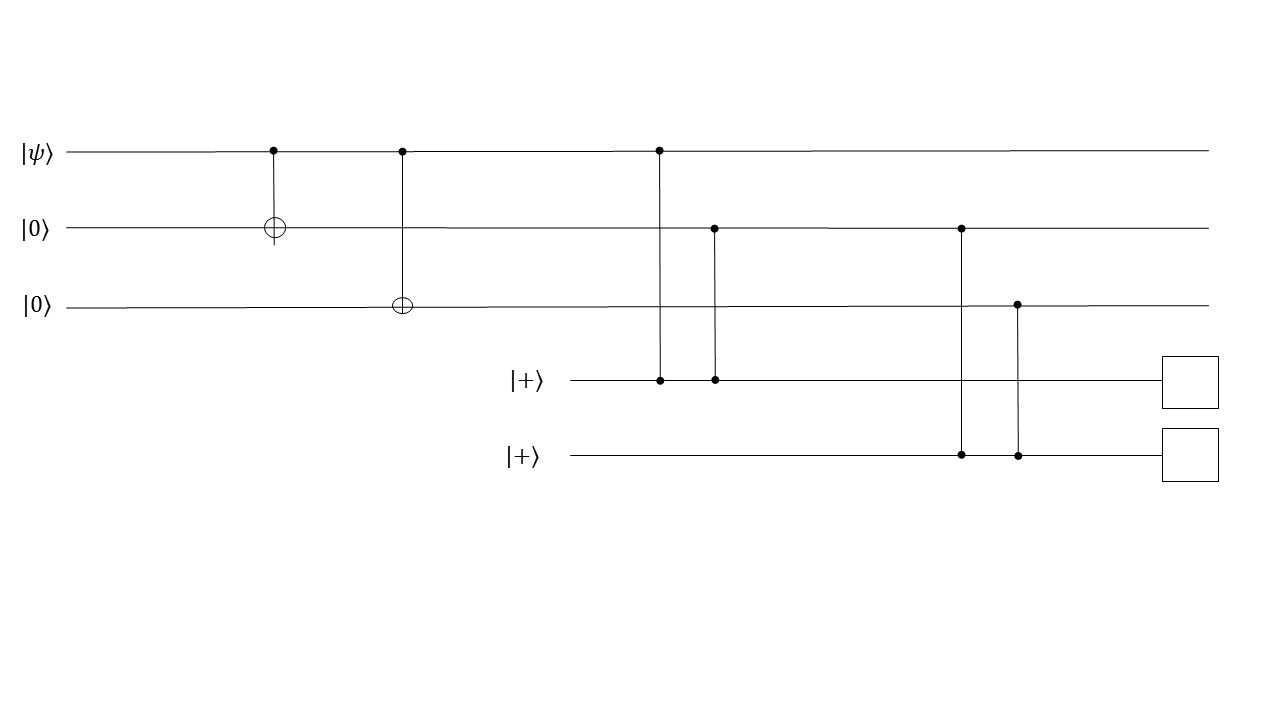
\includegraphics[width = \textwidth]{./Verification_Circuit.jpg}
\caption{Verification circuit.}
\end{figure}

Here, the line connected by two dots is the control $Z$ gate. It is symmetric between target and control qubits. We can only use the ancilla if both checks pass. This suppresses multi-qubit errors in the state \emph{and} keeps single qubit errors of order $p$. 

This is an example of \textbf{post-selection}. It is, in a sense, wasteful, but it is effective. 

To distinguish between $\ket{000} + \ket{111}$ and $\ket{000} - \ket{111}$, we inverse the circuit. Using the CNOT gates and measuring will give us either $\ket{+}$ or $\ket{-}$, which indicate the final state. 

Finally, while the above corrects for single or double errors in the preparation process, it still cannot correct for an $XXX$ error. However, we can easily repress it by repeating the measurement. For each time, we can measure three times and take the majority vote. This suppresses all errors to at least $p^2$. 

So, in summary, measurement errors can be suppressed by repeating the overall procedure. 

\section{State preparation}
Let us have a look at state preparation in fault tolerant measurements of stabiliser generators. For example, we will want a fault-tolerant measurement of $\bar{Z}$. 

Any unitary correction that we perform on  the state will automatically be transversal. The method we shall look at now is one of Steane's methods. Its prevalence was recently overtaken by topological codes. 

Note: for some reason I don't have many notes on this case. 

\section{Threshold example}
There are various things that we need to consider. 
\begin{itemize}
\item Different architectures and different error assumptions lead us to different thresholds. 
\item We can have analytic threshold which are rigorously proven, but they tend to underestimate the performance of the code (that, is we will always assume the worst-case scenario. 
\item Numerical thresholds are obtained by simulations. 
\end{itemize}


\subsection{Examples of thresholds}
The steane code has an analytic threshold of $ p = 10^{-5}$ and an analytic threshold of $p = 10^{-3}$. 

Other codes, such as the Bacon-Shor code, using a so-called subsystem code, have an analytic threshold of about $10^{-4}$. 

The surface code on the other hand has an analytic threshold of $10^{-1}$. 

\section{CSS code}
The Steane code is an example of a so-called Calderbank-Steane-Shor code (CSS). The basic idea is that the $X$ and $Z$ are independent. As we saw before, two classical codes are combined -- one to correct $X$ errors and one to correct $Z$ errors. 

Generators of stabilisers can be found where each generator contains either $X$ and $I$ tensor factors, or $Z$ and $I$ tensor products. 

CSS codes derived from this family are called \textbf{linear codes}. They are codes where codewords are formed as linear combinations, which means that they are linear in terms of basis codewords. 

As an example, we can look at the Hamming code: $(n = 7, k = 4)$. This code encodes the states into
\beq
\ket{0001} = \ket{0001011}
\eeq
\beq
\ket{0010} = \ket{0010110}
\eeq
\beq
\ket{0100} \rightarrow \ket{0100101}
\eeq
\beq
\ket{1000} \rightarrow \ket{100011}
\eeq
Here, the three last digits tell us about the parity of the code. 
Then, any permutation would be
\beq
\ket{0101} = \ket{0001} + \ket{0100} \rightarrow \ket{0101 110}
\eeq
where the above uses bitwise addition mod 2. In general, it implies htat 
\beq
abcd \rightarrow abcd (a + b + c)(a + c + d)(a + b + d)
\eeq
where the last few terms are indeed parity checks. Each codeword satisfy certainty parity conditions. Errors are detected by violations of these conditions. For example, the lst 3 bits plus the 1st bit of each codeword eaul zero. An error would be detected if these are found to not do so. 

For example, we can then encode these states in a matrix:
\beq
(1000111) \cdot x^T = 0
\eeq
We can write down parity constraints in a matrix, which is what we have done here. We then have a set of independent parity conditions. This turns out to be equivalent to the stabiliser generators! 

In particular, with a slight re-ordering of the bits, we see that the Hamming code has parity check
\beq
0001111, 0110011, 1010101
\eeq
So for each line $y$, we require $y \cdot x^T = 0$. We can check the errors by checking each line. This is where the stabiliser generator come from! 

CSS codes are constructed by mapping parity checks for a linear code to $X$-stabiliser generators and $Z$-stabiliser generators. 

In the Steane code, we had the transversal $T$ gate which is not in the Clifford group. Recall that 
\beq
S = \bpmat 1& 0 \\ 0 & i \epmat
\eeq
\beq
S^4 = I
\eeq
The Steane code codewords (see handouts) are very long. The Hamming weight for the states in the superposition is the same but for the first one $\ket{0000000}$. We now want to show that the $S$ gate is transversal. 

For the codeword $\ket{0}_L$ we have weights 0 and 4 for the codewords. For the codeword $\ket{1}_L$ we have weight 7 and 3. Thus, if we apply $\bar{S}$, 
\beq
( S^\dagger)^{\otimes 7} \ket{x} = -i)^{weight(x)} \ket{x}
\eeq
Note that $i^x$ obeys mod 4. So then, 
\beq
(-i)^{\otimes 7} \ket{0}_L = i \ket{0}_L
\eeq
\beq
(S^\dagger)^{\otimes 7} \ket{1}_L = (-1)^{3\mod 4} \ket{1}_L = i \ket{1}_L
\eeq

Similarly, there exists a 15-qubit code. Is has weight 8 on its codewords. Here, 
\beq
\bar{T} = (T^\dagger)^{\otimes 15}
\eeq
using the same argument. However, there is a bit problem for the 15-qubit code: It does not have a Hadamard gate! 

Finally, we can prove that it is impossible for a stabiliser code to have a universal set of gates. This is the \textbf{Eustin-Knill Thorem}. The best way to get around this is to use magic state distillation. 

\section{Magic state distillation}
The key idea here is to use \textbf{state injection}. Essentially, it will replace the pauli state preparation. We use the state $T \ket{+}$ as a resource to implement $T$ in the Clifford gates and Pauli basis. 

You can check the derivation for this yourself! 

The question now is how to fault-tolerantly prepare $T\ket{+}$. 

One way to do so would be to use fault-tolerant state preparation on the Steane code. This is called the Shor-scheme, see Nielsen and Chuang Section 10.6.2. However, the problem is that we get a very poor threshold. 

Here, we shall instead look at the magic distillation method. 

The idea is the following: We shall attempt to make $T\ket{+}$ without fault-tolerance. Consider a simple circuit that applies $T$ to the $\ket{+}$ followed by some error. The final state is not $T\ket{+}$ but rather some other mixed state $\rho$. We don't apply any error correction throughout the circuit. 

This error is generally unavoidable. Instead, we use magic state distillations. We take $N$ copies of $\rho$. We then measure a set of stabiliser generators on all of these states, then decode it to get $\rho'$. 

We can show that provided that $\rho$ is close enough to $T\ket{+}\bra{+} T^\dagger$, $\rho$ is good enough after distillation. 

This works for every code but the 15 qubit Reid-Miller-Code. Check Kitaev 2004 for a proof. They use the property that the $T$-gate is transversal for the 15 qubit code. 

These states are important because
\begin{itemize}
\item $T\ket{+}$ enables us to achieve universal quantum computing with the Clifford gates. 
\item Magic state distillation requires only Clifford group gates! 
\end{itemize}


Aside: Recall that stabiliser states form an octahedron in the Bloch Sphere. The this means tht we can convex closure of all points inside the octahedron. Just like we cannot obtain a pure state by convex combination of two mixed states, we cannot create $T\ket{+}$ from states inside the octahedron - $T\ket{+}$ lies outside it! 

We define the fidelity as
\beq
F = \sqrt{\bra{\psi} \rho \ket{\psi} }
\eeq
where
\beq
\ket{\psi} = \ket{\Psi}
\eeq
Then, define
\beq
1 - F^2 = \epsilon
\eeq
which is the distance between the obtained state $\rho$ and the desired state $\psi$. Magic state distillation works really well for the lower thresholds. See some Jupyter notebook notes with a numerical calculation on the Moodle website. 



\end{document}

